\documentclass[../main.tex]{subfiles}
\begin{document}
In the following chapter a general overview over the ECU structure is given, both in terms of hardware and software composition. The focus will be then directed towards the communications protocols and the standard used to develop software for \gls{ECU}s. 
\section{ECUs in a modern vehicle}
In the automotive industry there has been a remarkable evolution over the last few years in which embedded control systems have grown from stand alone control to highly integrated networked control systems \cite{Johansson_vehicleapplications}. In order to withstand this growth, there had been the need of creating higher scalability in the development process, via efficient communication protocols and standardize software development interfaces for the \gls{ECU}s.\\
The \gls{ECU} can be considered as the brain of the modern cars, based on a closed loop control system it outputs control commands to drive most of the vehicle capabilities.\\
In the logic of integrated networked control systems, the output arbitrated not only need to be logically correct, but need to abide time constraints. The complexity in both the control logic and the constraints related to the control increased both the hardware and software complexity in \gls{ECU}s.\\
In general in vehicles different control units are present, each responsible for the control of different tasks, the main ones are:
\begin{itemize}
    \item \gls{ECUM}, Engine control module, ensure the correct functionality of everything related to the power unit.
    \item \gls{BCM}, Brake control module, control the part related to break and breaking systems, such as \gls{ABS}.
    \item \gls{TCM}, Transmission control module, control the transmission.
    \item \gls{TCU}, Telematic control unit, control the \gls{HMI} and other user services offered by the vehicle. 
    \item \gls{SCM}, Suspensions control unit, control suspension, especially with upcoming technology related to active suspension control. 
\end{itemize}

\section{Hardware structure of an ECU}
\begin{figure}[h]
    \centering
    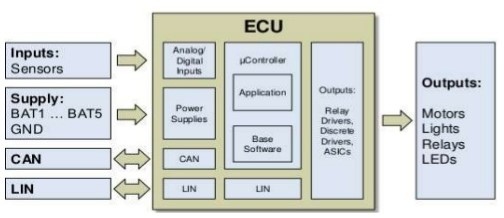
\includegraphics[width=\linewidth]{images_folder/electronic-control-unitecu-6-638.jpg}
    \caption{ECU structure}
    \label{fig:ECUHW}
\end{figure}
The hardware structure of an \gls{ECU} is a mixture of different electronics components, to better understand the overall organization, without entering to much in the electrical details a block scheme overview is offered by \ref{fig:ECUHW}.\\
It´s possible to easily differentiate between four different parts:
\begin{itemize}
    \item Power supply, handle the power input for the board and for the power components such as the motor driver or other power electronics components needed to drive the controlled parts. 
    \item Inputs, generic analog or digital inputs.
    \item Communications link, such as \gls{CAN} and \gls{LIN}.
    \item Outputs, output are directed to actuator, when the output pass through power electronics or can be the communication interface with other \gls{ECU}s.
    \item \gls{MPU}, Microprocessor unit and memory, in general Flash and \gls{RAM}. 
\end{itemize}
\section{AUTOSAR}
AUTomotive Open System ARchitecture (\gls{AUTOSAR}) is an open and standardize automotive software architecture, jointly develop by automobile manufacturers, supplier and tool developer. \gls{AUTOSAR} architecture was introduced to promote standardization of the software development process for Automotive Electronic Control Units. Prior to the introduction of \gls{AUTOSAR} \gls{ECU} software needed to be completely fitted around the hardware architecture, decreasing portability over different \gls{ECU} platforms and between different hardware producers. 
In order to address the problem \gls{AUTOSAR} introduced a an abstraction layer between the software and the hardware, thus ensuring that the software can be developed independently from the hardware. It is then \gls{AUTOSAR} task to make the two communicates together.
\begin{figure}[h]
    \centering
    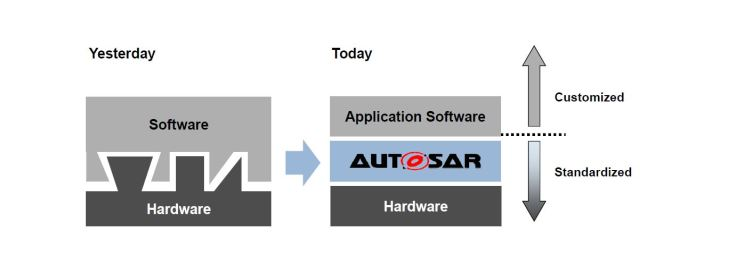
\includegraphics[width=\linewidth]{images_folder/autosarcapture.jpg}
    \caption{Autosar interface}
    \label{fig:AUTCA}
\end{figure}
\subsection{AUTOSAR Architecture}
The architectural structure of the \gls{AUTOSAR} standard is used to divide the hardware-independent software and the hardware-oriented software. Three main layers can be identified:
\begin{itemize}
    \item Application software, host all the functions that control the vehicle capabilities. In the \gls{AUTOSAR} language functions are also called \gls{SWC} (software components). An example of functions could be the software driving the windshield wipers. These software parts need to be able to receive a switch input in order to get triggered and give an output to light up the relative led on the cockpit dashboard.
    % first read
    \item Basic Software (\gls{BSW}), includes low level software like services and hardware specific software. Related to the previous example this gives the input output functionality required by the windshield wipers function. 
    \item Run-time Environment (\gls{RTE}), abstraction layer that manage the interface between the tow other layers. 
    \item Virtual Functional Bus (\gls{VFB}), this is an additional architectural strategy introduced by \gls{AUTOSAR} to decouple applications (windshield wiping) from the hardware infrastructure. The virtual bus map the two main type of communication between \gls{SWC} (intra-\gls{ECU} and inter-\gls{ECU}s) to the same function, allowing the user to simply define a communication, without having to bother about the protocol required (inter-\gls{ECU}s is generally based on \gls{CAN} while intra uses shared memory). The connection mapping is implemented by the RTE and becomes the concrete interface between individuals \gls{SWC} and between \gls{SWC}s and the \gls{BSW}.
\end{itemize}
\begin{figure}[h]
    \centering
    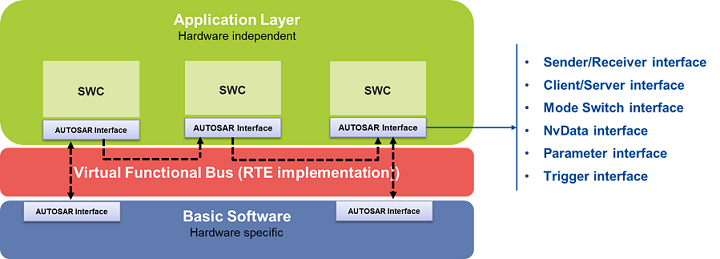
\includegraphics[width=\linewidth]{images_folder/878x-autosar_layers.b68.png}
    \caption{Autosar layers}
    \label{fig:AUTLAY}
\end{figure}
\subsection{Application Software Layer}
The application layer consist of the various software components interacting together. To connect software components, each component has well defined ports through which the component can communicate with other components or with Basic Software modules. The \gls{AUTOSAR} architecture defines two types of software components:
\begin{itemize}
    \item Application \gls{SWC}, implement an application. This \gls{SWC} type can use all the \gls{AUTOSAR} communication mechanism but can communicate to the sensors only via a Sensor-Actuator type software component. 
    \item Sensor-Actuator type \gls{SWC}, has access to \gls{ECU} specific hardware \gls{I/O} signals. This \gls{SWC} is responsible for reading a sensor and provide its data to other components or to set the status of an actuator. 
\end{itemize}
The \gls{SWC} communicates via Ports. A port is used to send or request information. Once a port is defined it needs to be associated with the interface that define the information exchange. The main interfaces that are supplied by \gls{AUTOSAR} are the following:
\begin{itemize}
    \item Sender/Receiver, defines a set of data elements that are sent from one components to another. 
    \item Client/Server, a server can implement a set of operation and make the result available to the clients. This work as a function call for the clients. 
    \item Parameter interface, define a set of parameters (constant or calibrate)
    \item Non-volatile data access, provides access to Non volatile data. 
    \item Trigger interface, give a \gls{SWC} the ability to trigger another \gls{SWC}. This works as an interrupt. 
    \item Mode-Switch, activate particular modes of use. 
\end{itemize}
\subsection{SWC structure - AUTOSAR Internal Behaviour}
Every \gls{SWC} is not just composed by runnable code, in order to withstand the \gls{AUTOSAR} standard a certain architecture need to be implemented in every \gls{SWC}. The main \gls{IB} elements of an SWC are the following:
\begin{itemize}
    \item Runnables, these are the pieces of code which implement the \gls{SWC} functionality. A single \gls{SWC} can have multiple runnables. 
    \item RTE-Event, in real time environment such as the \gls{ECU} the scheduling information of an SWC, its priority and frequency of execution need to be defined. Those can be found inside the RTE-Events. 
    \item Access Point, the access point specify how each runnable expect to access the information conveyed through the \gls{SWC} connection interfaces. 
\end{itemize}
\subsection{Example implementation of a windshield wiper control}
Having defined the \gls{AUTOSAR} standard structure, it´s useful to define an example of implementation to better understand. Consider the function windshield wiping. The function graphical structure can be defined as follows:
\begin{figure}[H]
    \centering
    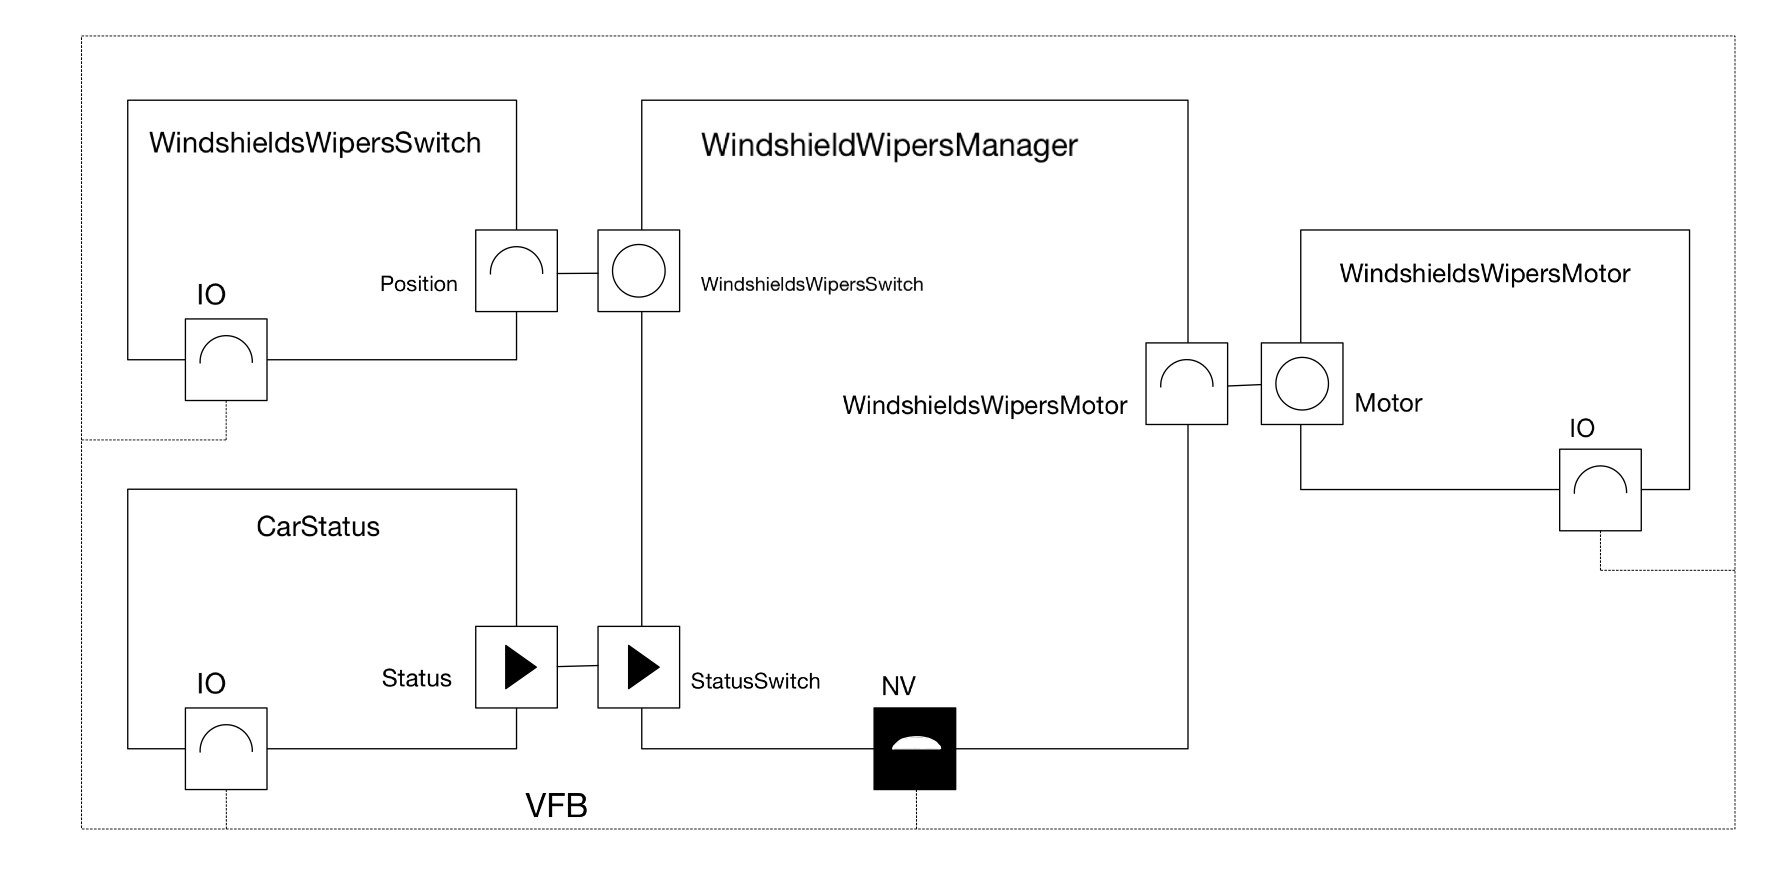
\includegraphics[width=\linewidth]{images_folder/windshield_WIpers_aUtosar.jpeg}
    \caption{Windshield wipers implementation}
    \label{fig:WINWIP}
\end{figure}
The contains tree instances of the Sensor-Actuator \gls{SWC}. The first is the sensor reading the status of the \textit{WindeshieldsWipersSwitch}, the read is done via the \gls{I/O} labeled port. The status is transmitted via a service. The other sensor, \textit{CarStatus} instead check the status of the vehicle, on weather or not this is on or off. The transmission is done via a sender receiver. The main difference between the two is that the server/client configuration that the data from a server is only available to the client requesting the data. Instead a receiver/sender configuration the data is "published" on the \gls{RTE}, and the connected receiver/writer can access/modify the data.\\
The only actuator \gls{SWC} is the one in charge of controlling the windshield wipers motor, \textit{WindshiedsWipersMotor}. The managing component, \textit{WindshieldWipersManager} is the one who compile the logic of the actuation. It is client of the Switch, and can therefore request the status (the request periodicity is defined by it´s RTE event element). Based on it and on the information from \textit{CarStatus} define an actuation that is given as service to the client \textit{WindshieldsWipersMotor}. The managing components also have a \textit{Nvblock} which allow it to save its internal state to the non volatile memory. 
The design can be done avoiding entering in \gls{ECU} specific details. To create a real application two more steps are required. The first one is to define the managing block behaviour through an executable and the second one is the passage from \gls{VFB} communication to real \gls{ECU}, exiting the \gls{AUTOSAR} layer of abstraction and entering in more \gls{ECU} specific details. This is done by the run-time environment.
Communication on the ECU is done via the use of a shared \gls{bus}, using the \gls{CAN} communication protocol. The details of the communication interface are defined in the following section.

\subsection{CAN - Communication protocols in ECU}
\gls{CAN} is the main communication protocol used in the automotive field. \gls{AUTOSAR} run-time environment is responsible of connecting the \gls{AUTOSAR} scheme with the \gls{CAN} capabilities related to the \gls{ECU} hardware.\\
The Control Area Network (\gls{CAN}) is a serial communication protocol suited for networking sensors, actuators and other nodes in real-time systems. \gls{CAN} define the protocol of communication for two of the layer of \gls{OSI}, Open System Interconnections, an abstraction model for communication protocol. 
\begin{figure}[H]
    \centering
\begin{tikzpicture}[box/.style={on chain,join,draw,minimum width=4cm,minimum height=1cm,
align=center},start chain=going below, node distance=5mm,font=\sffamily,fbox/.style={draw,thick,fill=white}]
  \node[box] (a) {Application layer};
  \node[box] (b) {Presentation layer};
  \node[box] (c) {Session layer};
  \node[box] (d) {Transport layer};
  \node[box] (e) {Network layer};
  \node[box] (f) {Data Link layer};
  \node[box] (g) {Physical layer};
  \node[above=1cm, xshift=1mm] (l) {Application A};
  \begin{scope}[on background layer]
   \node[fbox,fit=(a|-l.north) (g),inner xsep=3mm] (f1){};
  \end{scope}
\end{tikzpicture}
    \caption{OSI}
    \label{fig:ECUstructure}
\end{figure}
\gls{OSI} is an abstraction model for the communications protocols that describe the communication processes in a abstract manner. The description starts from the physical layer, which is the one relate to the physic of sending a message all the way to the Application layer, that defines what need to be done with the actual message. The layers in which \gls{CAN} introduces a standardization are the Physical layer and the Data link layer.\\
The physical layer is indeed composed by the physical transport media, from cables plugs and sockets. \gls{CAN} uses a twisted pair in which the differential voltage between the couple represents the bits transmitted. The Data link layer defines instead the \gls{MAC}, Media Access Control Methods. In \gls{CAN} this is set to \gls{CSMA/CA} or Carrier Sense Multiple Access/ Collision Avoidance. This complex series of acronyms define the simple concept that on a \gls{CAN} \gls{bus} a message can be sent only if the \gls{bus} is free, in case two nodes start sending a message at the same time, then the message with the highest priority win and the node with the low priority message retrieve to a receiver status.
\subsubsection{CAN message format}
\begin{figure}[H]
    \centering
    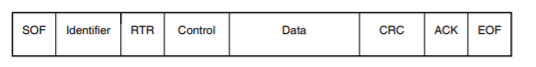
\includegraphics[width=\linewidth]{images_folder/can message.png}
    \caption{CAN message structure}
    \label{fig:CANMSG}
\end{figure}
\gls{CAN} distinguish different message formats, the main one is the data frame format, which is used to send logical information. The data frame is composed by:
\begin{itemize}
    \item \gls{SOF}, start-of-frame, which denotes the start of the transmission. The length is 1 bit. 
    \item Identifier, the 11 bit identifier is used not only to identify the message but to define its priority. 
    \item \gls{RTR}, remote transmission request, define the difference between a message sent and a remote request. 
    \item Control bits, consist of 6 bits and define how many bytes of data follow in the data field. In theory not all of the 6 control bits are used to identify the length of the data, since this one is limited to a maximum of 8 bytes. With that being said the actual number of bits reserved to define the data length is 4, which is a bit more than necessary. This is done to allow controller to send data which is more than 8 bytes (9 - 15) in special cases.
    \item Data, actual data to be sent, with a maximum of 8 bytes ($64$ bits = maximum value that can be sent is $2^{64} - 1$).
    \item \gls{CRC}, cyclic redundancy checks, enable the receiver to check if the received bits have been corrupted. The techniques used are bit monitoring and bit stuffing.
    \item \gls{ACK}, consist of a two bit acknowledgement used by the transmitter to receive an acknowledgment of validity form the receiver.
    \item \gls{EOF}, end-of-frame, is a seven bit signal that define the end of communications. 
\end{itemize}
\subsubsection{CAN arbitration}
Arbitration is the mechanism that handle \gls{bus} access conflict. As already underlined when describing the can Data link layer, based on collision avoidance every node can start sending if the \gls{bus} is free. In the case in which two nodes start the communication simultaneously arbitration comes into place, resolving the conflict. During the arbitration phase each transmitting node send the identifier and compares it with the other by motoring the level of the \gls{bus}. Whenever a node sense a dominant level on the bus, while sending a recessive one, than the node stop the communications and start listening to the \gls{bus} (become a receiver). In \gls{CAN} a recessive level is couple with the bit 1, while a dominant with 0. Consider having three nodes with the following identifiers:
\begin{equation}
I_{1} = 11001101010
\end{equation}
\begin{equation}
I_{2} = 11001011011
\end{equation}
\begin{equation}
I_{3} = 11001011001
\end{equation}
\begin{figure}[ht]
    \centering
    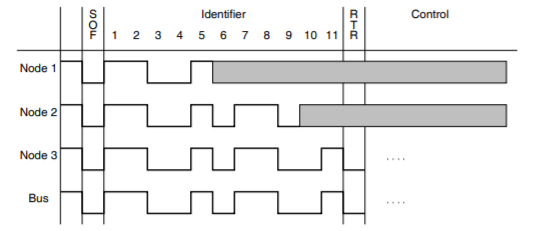
\includegraphics[width=\linewidth]{images_folder/can_arbitration.png}
    \caption{CAN arbitration}
    \label{fig:CANABR}
\end{figure}
As exemplified in \ref{fig:CANABR} the nodes starts by sending the \gls{SOF}, then the identifier comes into play. The nodes continue sending on the \gls{bus} their identifier until a collision happen. After five bits where all the node have equal identifier, at bit number 6 the $I_1$ set the bus on a recessive level while sensing both from $I_2$ and $I_3$ a dominant level, therefor $I_1$ stop the communication and switch to a receiver mode. Therefor $I_2$ and $I_3$ continue sending on the \gls{bus}. The tenth bit of $I_2$ is at recessive level while $I_3$ is at dominant. Node $I_3$ is the transmitter and therefor continue with the transmission of the other part of the data frame while $I_2$ becomes a receiver, thus completing the arbitration process.\\
\gls{CAN} is affected by starvation´s problems. Low priority nodes may expect large latency in case of high priority units being very active. \\
It´s important also to underline the fact that there is no message destination address in \gls{CAN}, instead each node picks up all the traffic on the bus.\\
From and electrical standpoint \gls{CAN} arbitration mechanism work as follow. Consider the example in Fig. \ref{fig:CANABRELT} where \gls{CAN} nodes are exemplified by open collector transistors. 
The level of the bus is at a low level (dominant) in the case in which just one of the of transistor in the network output a dominant level. This is also the explanation of why zero is dominant, only one transistor is needed in a closed configuration an the whole bus sees a zero on it independently by the status of other transistor. The bus will only be at high level (recessive) when all the transistors in the network output a recessive level or the transistors are all open, putting 1 on the \gls{bus}.
\begin{figure}[ht]
    \centering
    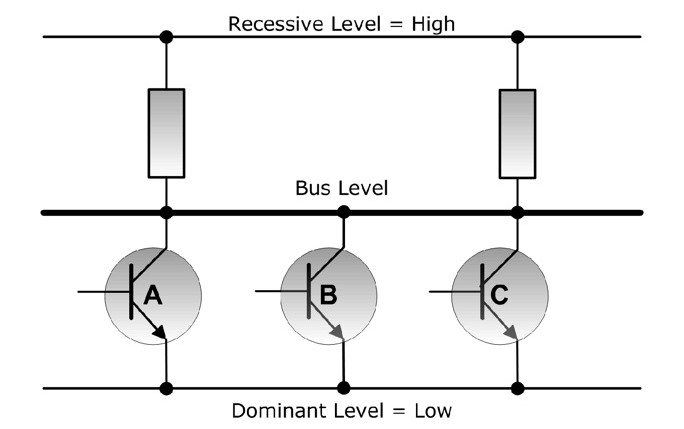
\includegraphics[width=0.7\linewidth]{images_folder/controller-area-network-can-bus-bus-arbitration-3.jpg}
    \caption{CAN Arbitration -  electrical scheme}
    \label{fig:CANABRELT}
\end{figure}

\section{Model based design}
\subsection{Introduction}
Inside the automotive world the trend that has drawn more differences in the way car are constructed is in the electronic components side. if the cost related to the development of mechanical components, safety features and logistic increased constantly through the years, the cost related to the electronic components exponentially increased. What once was a mechanical system is most probably going to be a embedded system nowadays. The increase in hardware related to embedded components requires an increase in the software in order to control it. The yearly increase in lines of code for car is a statement in support of the importance of software. 
% \begin{figure}[H]
%     \centering
%     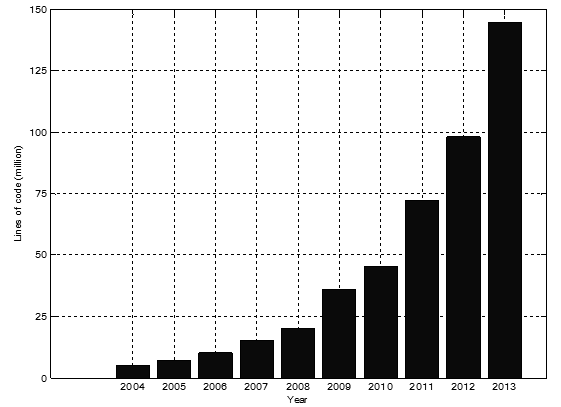
\includegraphics[width=\linewidth]{images_folder/Yearly-increase-in-automotive-software-complexity-shown-by-million-lines-of-code-of-1-ConvertImage.png}
%     \caption{Yearly increase in automotive software complexity}
%     \label{fig:yearlyincreas}
% \end{figure}
Software development therefor faces new challenges, related to shorten development time, a high need of scalability  not only in the software but also in the development platforms, complex safety requirements and adaptability over continuously changing hardware.\\
Model based design has entered the automotive conversation because it can full fill the previously reported challenges. The model based approach brings two main characteristic to the table: on the one hand it gives a development platform which is component independent, therefor allowing for better integration through rapidly changing hardware, on the other hand makes the integration of new features not time depended. In this sense it recall a concept similar to Scurm, where changes are welcomed during the whole development process. in this case, with model based design, changes are welcomed during the whole life of the software.
\subsection{Model based design}
Model-Based Design provides a mathematical and visual approach to develop complex control and signal processing systems. It centers on the use of system models throughout the development process for design, analysis, simulation, automatic code generation and verification \cite{Mathworks}. The main features are abstraction and automation. As reported by \cite{modelbased} model based tackle complexity via abstraction and automation. Abstraction is achieved by the using suitable models of a software system, while automation is achieved by systematically transform these models into executable source code.\\
Engineers create a model to specify the behavior of an embedded system; the model, which consists of block diagrams, textual programs, and other graphical elements, is an executable specification that lets engineers run simulations to test ideas and verify designs throughout the development process. The main advantages are
\begin{itemize}
    \item The design can be tested, refined and retested throughout the development process, thus increasing product quality. Test and validation are done continuously rather than at the end of the process. Error can be found before hardware is required for testing
    \item Simplification of complex system, by providing a graphical design models simplify the creation of high complexity functions, especially when compared with hand code components. This advantage as it enhance and simplify communication inside the team, as it is easy to understand the models. 
    \item Embedded code can be generate automatically from the models. To adapt the model to different hardware there´s the need to adjust the compiler, not every single model. This allow for great adaptability to rapidly changing hardware. 
\end{itemize}

\cleardoublepage
\end{document}
